\subsection{Results on M2}
We tested StarNet on the SDSS image of M2, a crowded starfield found in run 2583, camcol 2, and field 136.
M2 was also imaged in the ACS Globular Cluster Survey~\cite{Sarajedini_2007}
using the Hubble Space telescope (HST),
which has $\approx20$ times the angular resolution and $\approx30$ times the exposure of the Sloan telescope. The reported catalog from this Hubble survey was used as ground truth to 
validate our results.

We focused on a specific $100 \times 100$ subimage of M2 that \cite{Portillo_2017, Feder_2019} cataloged using PCAT.
This subimage is located $\approx2$ arcseconds away from the heavily saturated core of the cluster;
even in this subimage, the HST catalog contained over 1000 stars brighter than the 22nd magnitude in its F606W band.

\subsubsection{Runtime} 
\label{sec:runtime}
We tiled the $100\times 100$ image into $2\times 2$ tiles. The neural network inputs were the $2\times2$ tiles padded by three pixels (see Figure~\ref{fig:starnet_arch}). 
We ran the initial sleep phase~\eqref{eq:sleep_phase_summary}
% \jeff{What does it mean to ``train'' a sleep phase?}
with the PSF and background set to SDSS estimates. We trained for 200 epochs with 200 images per epoch with  
the Adam optimization routine~\cite{kingma2014adam}. 
% \jeff{The defaults are specific to PyTorch, not Adam. If you are going to talk about the hyperparameter settings, at least say what ``default'' means.}
% \jeff{That said, it's probably better not to mention how you set the parameters---too much detail. The reader will trust that you did something reasonable, and they can check out your open source code if they want this level of detail.}
On a single Nvidia GeForce RTX 2080 Ti GPU 
the initial sleep phase took approximately 10 minutes. 

We ran two further wake-sleep cycles. Each cycle took approximately a minute. The subsequent sleep phases were shorter (10 epochs with 200 images each), and the wake phase employed SGD, with the gradient estimator in \eqref{eq:mstep_grad}. 

After training, evaluating the approximate posterior on the $100 \times 100$ image of M2 took $\approx 0.2$ seconds. 
By comparison, the reported runtime of PCAT, which uses MCMC, is 30 minutes on the same $100 \times 100$ image~\cite{Feder_2019}. 

We emphasize that the speed of our procedure at inference time (which excludes training time) enables our method to scale up to large astronomical surveys. A single SDSS image is $1489 \times 2048$ pixels. Projecting the reported runtime of PCAT to the full image, 
we would expect a runtime of 
$\approx 30\text{min} \times 14 \times 20 = 8400$min, or almost six days. 
\jeff{What would be the runtime of PCAT for all of SDSS? You can get the relevant information about SDSS here: \url{https://www.sdss.org/dr13/scope/}.
It might be information to do this calculation for LSST too. (See lsst.org)
}
\bryan{So SDSS has about one million images. 
6 days times one million gives about 16000 years ... is this too extreme to even report?}

In contrast, if we assume the PSF and background are homogeneous 
across the full SDSS image (which PCAT also assumes), we can 
train our variational approximation using wake-sleep 
on a small $100 \times 100$ subimage
(while getting estimates of the PSF and background along the way),
a one time computational cost of twelve minutes. 
Producing a catalog on the full $1489 \times 2048$ image will require 
$\approx 0.2\text{sec} \times 14 \times 20 = 56$ seconds. In practice, 
this will be even faster as we would batch the image tiles to run in parallel on a GPU. 

Moreover, an SDSS image is indexed by a run, camera column (camcol), and field.
A run is one continuous scan of the telescope, usually corresponding to one night of data collection. 
A run is broken down into fields; some runs have over 800 fields. 
Each field contains six camera columns. 
Thus, for a large-scale sky survey like SDSS which 
consists of over 8000 runs for a total of nearly one million images, MCMC will be infeasible. 


\subsubsection{Inference}
\label{sec:m2_results}
We compared StarNet with PCAT and DAOPHOT~\cite{stetson2987daophot}. DAOPHOT is an algorithmic routine designed for crowded starfields. 
To detect stars, the observed image is convolved with a Gaussian kernel. 
The convolved image is scanned for peaks above a given threshold, which are then labeled as stars. The DAOPHOT catalog of M2 was reported in 
\cite{An_2008_m2}. While DAOPHOT returned photometry for all five SDSS bands, 
we chose to model only the $r$ and $i$ bands for StarNet and PCAT. We found that for StarNet and PCAT, the inclusion of more bands did not significantly improve
the quality of our detections on metrics defined below. 

Both DAOPHOT and the Hubble survey reported a ``traditional" catalog, that is, a list of stellar locations, fluxes, and 
error bars nominally representing marginal uncertainties.
\jeff{Do these catalogs contain any uncertainty estimates?}
In the context of probabilistic cataloging (StarNet and PCAT), the posterior 
defines a distribution over catalogs -- each draw from the posterior returns a catalog 
(of potentially varying length) of stellar locations and fluxes. 

Given an estimated catalog, three metrics we examined were the true positive rate (TPR), the positive predicted value (PPV), and the F1 score. Using the HST catalog as ground truth, the TPR is the proportion of stars in the HST catalog that had a match in the estimated catalog;
the PPV is the proportion of stars in the estimated catalog that had a match in the HST catalog. Like \cite{Portillo_2017, Feder_2019}, we defined a match to be when the estimated location and the HST location were within 0.75 pixels
(TODO: use 0.75 because that's what PCAT did. Results actually right now are for 0.5 pixels),
and the estimated $r$-band flux and the HST F606W band flux were within half a
magnitude. The slack in the magnitude allows for some discrepancy between the 
SDSS $r$-band and the the Hubble F606W band. The Hubble F606W band absorption range is broader than the SDSS $r$-band, though they centered at roughly the same wavelength. Finally, the F1 score is defined as the geometric average between the PPV and the TPR. 

We filtered the Hubble catalog to stars brighter than 22.5~mag in the F606W band, corresponding to the detection limit of point sources in SDSS images. In our method and PCAT, this amounted to setting $f_{min}$ in the flux prior (equation~\ref{eq:flux_prior})
to the 22.5th magnitude; all dimmer stars were absorbed into the sky intensity. 

Table~\ref{tab:summary_stats} reports the PPV and TPR for the considered cataloging methods.
% \jeff{Summary statistics of what? Could you say something like ``Table~\ref{tab:summary_stats} reports the performance of these methods'' instead? That would be more descriptive.}
For StarNet, the TPR and PPV were computed at the maximum a posteriori (MAP) catalog under
the variational distribution. For PCAT, the TPR and PPV were computed for each catalog sampled from their posterior and averaged over 300 posterior samples. 

\jeff{A lot of sentences that have ``we'' as the subject can be rewritten in way that doesn't mention us (without switching to passive voice, which often doesn't sound good). It makes the writing easier to understand because typically ``we'' are not really central to the idea we're trying to convey. 
So you might say thing like ``Our method performed better than PCAT in terms of TPR and PPV'' rather than all four of the follow sentences: ``We compute the the TPR and PPV for our method. We compared it to PCAT. We found that our method performed better than PCAT. Note that we used the MAP estimate to compute TPR.''
}
Training StarNet using only the sleep phase, that is optimizing~\eqref{eq:sleep_obj} at the SDSS estimates of the model parameters, returned 
a MAP catalog with a TPR of 0.52 and PPV of 0.45. Two further cycles of wake-sleep training improved the PPV to 0.62; the TPR decreased slightly to 0.49. The catalog did not noticeably improve after the second iteration of wake-sleep. The wake-sleep PPV was also better than PCAT by 0.26. Furthermore, the TPR of PCAT
only improved by 0.02 over wake-sleep, even though PCAT predicted roughly 50\% more stars than wake-sleep. 
% , and ran 
% a first sleep phase (optimizing equation~\ref{eq:sleep_obj}). We compare the 
% catalog obtained under the MAP estimate under the variational distribution trained using only this sleep phase against the 
% variational distribution obtained after two further cycles of wake-sleep. 
% We define the ``wake-sleep" catalog 

% Our  MAP  estimate  under  the  variational  distribution  trained  using  wake-sleep
% (which we will call our “wake-sleep catalog”) had similar TPR to the 


% (which we will call our ``wake-sleep catalog")


Conversely, the DAOPHOT catalog detected the fewest number of stars, and it had the lowest TPR of all the methods.
Further, while wake-sleep predicted nearly three times as many stars as DAOPHOT, wake-sleep only suffered a decrease in PPV of 0.04. 

% We combined TPR and PPV into one statistic using the F1 score,
% defined as the geometric average between TPR and PPV, and found that both sleep-only and wake-sleep outperform PCAT and DAOPHOT.

% \begin{table}[!tb]
% \centering
% \caption{Performance metrics on M2.
% For probabilistic methods (StarNet and PCAT)
% the ``\#stars" column refers to the mean number of stars under the (approximate) posterior, while the right-most column displays the 5-th and 95-th percentiles under the posterior. }
% \label{tab:summary_stats}
% \begin{tabular}{l|ccc|cc}
% \toprule
%      Method &   TPR &   PPV &  F1 score &  \#stars & (q-5\%, q-95\%)\\
% \midrule
%     DAOPHOT &  0.20 &  0.63 &      0.30 &     295 & -- \\
%        PCAT &  0.56 &  0.40 &      0.47 &    1672 & (1664, 1680)\\
%  Sleep-only &  0.51 &  0.47 &      0.49 &    1292 & (1260, 1324)\\
%  Wake-sleep &  0.51 &  0.60 &      0.55 &     1014 & (987, 1041)\\
%      %Hubble &  1.00 &  1.00 &      1.00 &     1114 & -- %\\
% \bottomrule
% \end{tabular}
% \end{table}

\begin{table}[!tb]
\centering
\caption{Performance metrics on M2.
For probabilistic methods (StarNet and PCAT)
the ``\#stars" columns provide the mean along with the 5th and 95th percentiles
for the number of stars under the (approximate) posterior,
The number of stars in the Hubble catalog is 1114. }
\label{tab:summary_stats}
\begin{tabular}{l|ccc|cc}
\toprule
& & & & \multicolumn{2}{c}{\#Stars} \\
     Method &   TPR &   PPV &  F1 score &  mean & (q-5\%, q-95\%)\\
\midrule
    DAOPHOT &  0.20 &  0.65 &      0.31 &     357 & -- \\
       PCAT &  0.55 &  0.37 &      0.44 &    1672 & (1664, 1680)\\
 StarNet (our) &  0.53 &  0.48 &      \textbf{0.50} &    1462 & (1430, 1497)\\
\bottomrule
\end{tabular}
\end{table}


Figure~\ref{fig:summary_stats} shows the TPR and PPV binned by magnitude.
Wake-sleep and PCAT showed similar TPR across all magnitudes; both were
uniformly better than DAOPHOT. Wake-sleep had a PPV higher than PCAT for all magnitudes. 
\begin{figure}[ht]
    \centering
    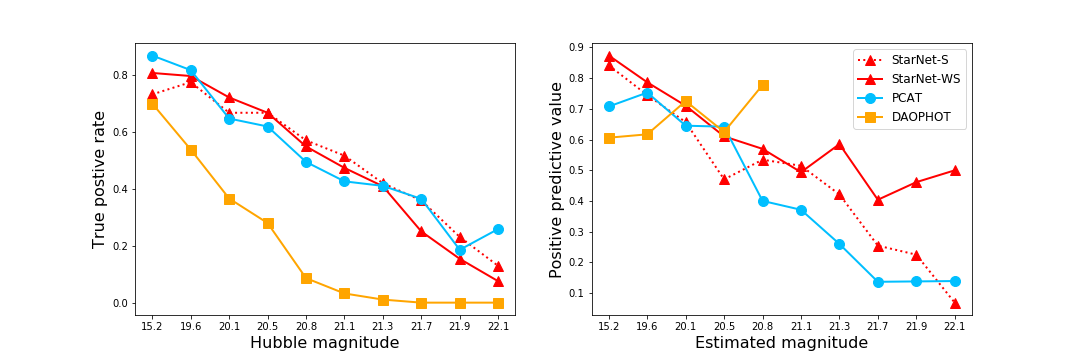
\includegraphics[width=0.99\textwidth]{figures/summary_statistics_m2.png}
    \caption{True positive rate and positive predicted value of various cataloging
    procedures on M2, plotted against magnitude percentile.
    Smaller magnitudes correspond to brighter stars. }
    \label{fig:summary_stats}
\end{figure}


Figure~\ref{fig:example_subimages} shows four $10\times10$ subimages, and overlays the wake-sleep MAP catalog on the Hubble catalog. The DAOPHOT catalog and one catalog sample from PCAT are also shown. 

Figure~\ref{fig:example_subimages_sampled} shows sampled catalogs from both our wake-sleep approximate posterior as well as from PCAT.
Our variational approximate posterior appeared to show larger uncertainties
than PCAT. 
\newpage

\begin{figure}[H]
    \centering
    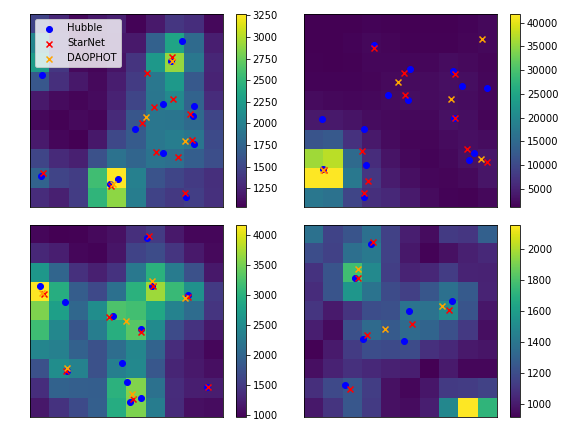
\includegraphics[width=0.49\textwidth]{figures/example_subimages_ws.png}
    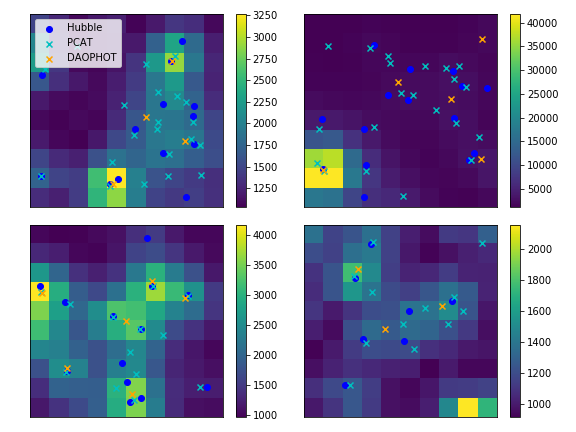
\includegraphics[width=0.49\textwidth]{figures/example_subimages_pcat.png}
    \caption{Estimated catalogs on four 10$\times$10 subimages from
    M2. Blue dots are Hubble stars brighter than the 22nd magnitude.
    Wake-sleep, PCAT, and DAOPHOT estimated stars are in
    red, cyan, and orange x's, respectively. }
    \label{fig:example_subimages}
\end{figure}
\newpage

\begin{figure}[H]
    \centering
    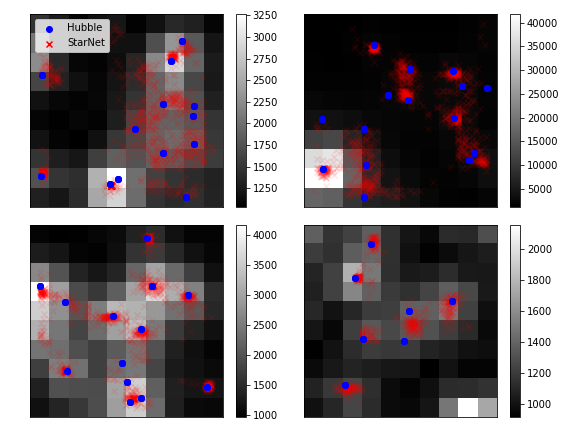
\includegraphics[width=0.49\textwidth]{figures/example_subimages_samples_ws.png}
    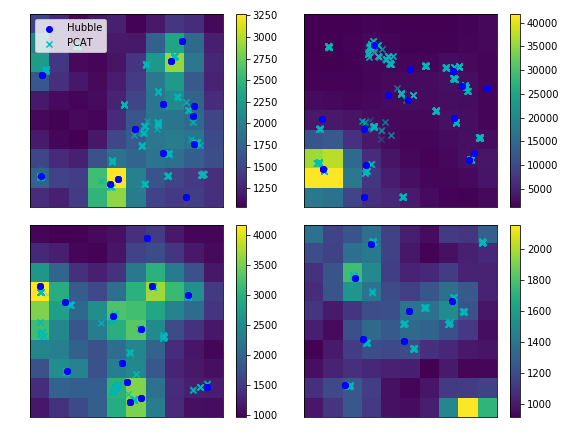
\includegraphics[width=0.49\textwidth]{figures/example_subimages_samples_pcat.png}
    \caption{Four 10$\times$10 subimages from
    M2. Blue dots are Hubble stars brighter than the 22nd magnitude. (Left) Posterior samples from the wake-sleep variational
    posterior and (right) posterior samples from the MCMC chain of PCAT. }
    \label{fig:example_subimages_sampled}
\end{figure}
\newpage

Figure~\ref{fig:z-score_calibration} examines the calibration of the uncertainties under StarNet. We evaluated the wake-sleep approximate posterior 
conditional on the true number of stars in the Hubble catalog. 
Thus, each star in our estimated catalog was matched with exactly one Hubble star
by finding the permutation of Hubble stars that had the largest log-likelihood under our variational distribution $q_\eta$. For each star, we computed the z-score $(y - \hat y) / \hat \sigma$, where $y$ is the true log-flux or 
logit-location; $\hat y$ is the mean of the Gaussian variational distribution, and $\hat\sigma$ the standard deviation.
If the uncertainties were perfectly calibrated, the distribution of the z-scores would be a standard Gaussian. 
In Figure~\ref{fig:z-score_calibration}, the tails of our empirical z-score distribution are slightly larger than standard Gaussian, suggesting that our error is somewhat under-estimated. 

\begin{figure}[ht]
    \centering
    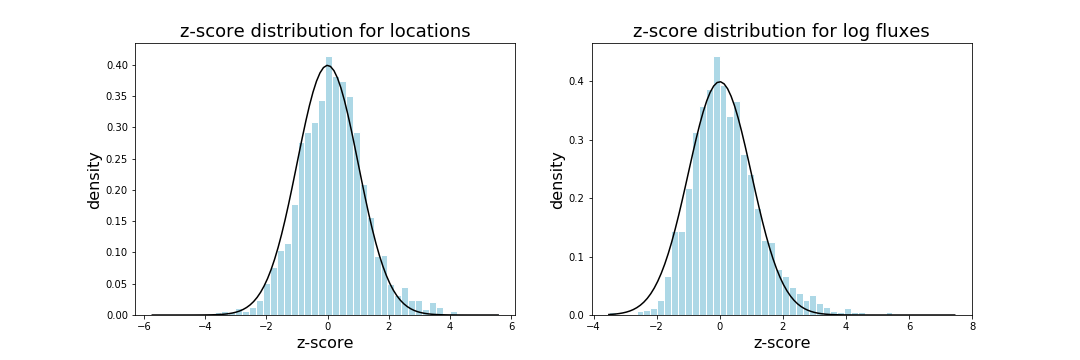
\includegraphics[width=0.99\textwidth]{figures/z-score_calibration.png}
    \caption{The calibration of uncertainties in the wake-sleep variational posterior. 
    Conditional on the true number of stars, displayed are histograms of the z-score of the true logit-location or log-flux evaluated at our variational posterior. 
    The empirical mean and variance for the logit-location z-scores are 0.27 and 1.91, respectively; the empirical mean and variance for the log-flux z-scores are 0.17 and 1.53, respectively. 
}
    \label{fig:z-score_calibration}
\end{figure}

Figure~\ref{fig:luminosity_fun_m2} shows the distribution of estimated $r$-band fluxes. We compared them 
with the distribution of F606W-band fluxes in the HST catalog. While the Hubble F606W-band has a broader absorption range than the SDSS $r$-band, they are centered at roughly the same wavelength. For PCAT, we displayed the flux distribution from a single catalog sample; for our wake-sleep variational 
posterior, we used the MAP catalog. DAOPHOT returned fluxes only up to $\approx21$ mag.
Conversely, PCAT greatly over-estimated the number of dim stars with magnitude less than 21 mag. Our flux distribution came closest to the distribution of the HST catalog. 

\begin{figure}[ht]
    \centering
    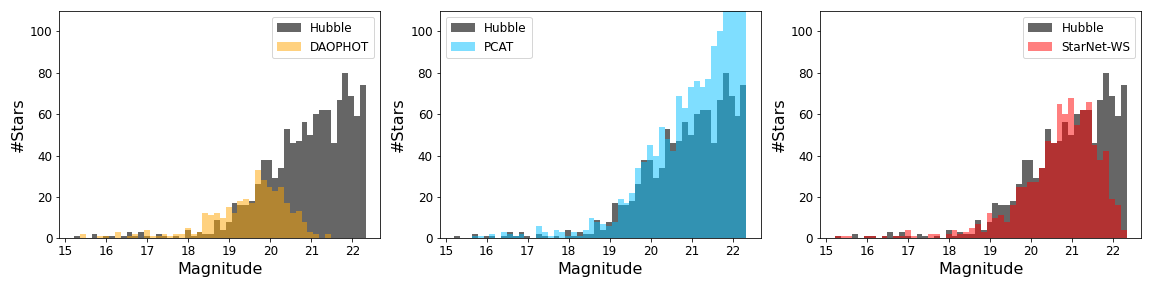
\includegraphics[width=0.99\textwidth]{figures/luminosity_fun.png}
    \caption{Source magnitude histograms on M2. }
    \label{fig:luminosity_fun_m2}
\end{figure}

Finally, Figure~\ref{fig:cmd_m2} displays the estimated color-magnitude diagrams. While the Hubble F606W-band corresponds roughly to the SDSS $r$-band, there is no such correspondence for the SDSS $i$-band. Thus, using the Hubble locations, we estimated the ``true" $i$-band fluxes using maximum likelihood. Letting $x^{(i)}$ be the SDSS image in the $i$-band, $N_H$ the number of stars in the Hubble catalog and $\ell_H$ their locations, we found  
\begin{align}
   f^{(i)}_H = \argmax_{f\in\mathbb{R}^{N_H}} \log p(x^{(i)} | N_H, \ell_H, f)
   \label{eq:optim_iband_flux},
\end{align}
where the log likelihood is given by~\eqref{eq:loglik}. We used the estimated $i$-band fluxes and the reported Hubble F606W-band fluxes $f_H^{(r)}$ to define the ``true" colors, defined as $2.5\log(f_H^{(i)}/f_H^{(r)})$. We compared
the color-magnitude diagram found from Hubble parameters with catalog returned by DAOPHOT, PCAT, and wake-sleep. We see that DAOPHOT did not capture the full spectrum of colors; of all three methods, PCAT seemed to best capture the color spectrum. All three methods however, were able to capture the arm thing (TODO there is a name for this ... main sequence turnoff?) that branches off at low magnitudes. 

\begin{figure}[ht]
    \centering
    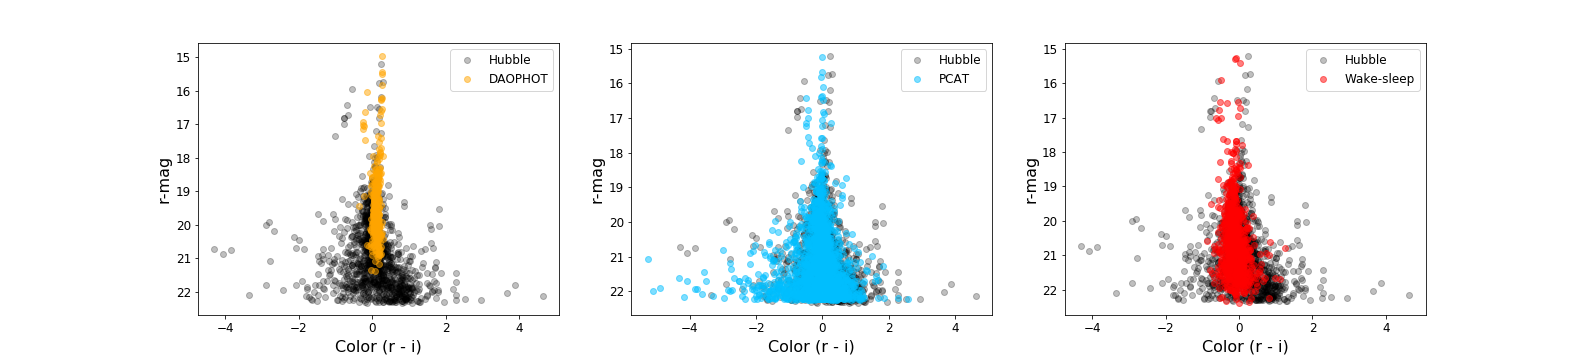
\includegraphics[width=0.99\textwidth]{figures/cmd.png}
    \caption{Color magnitude diagrams on M2. }
    \label{fig:cmd_m2}
\end{figure}


\subsubsection{Estimation of model parameters}
\label{sec:results_model_params}
In this section, we examine our estimated parameters 
for the sky intensity and the PSF. As shown in the previous section, wake-sleep improved the catalog over sleep-only on the F1 score. In Table~\ref{tab:chi-square-stats1}, we
print the negative log-likelihood $- \log p_\phi(x | N_{H}, \ell_{H}, f_{H})$ for various model parameters $\phi$, where $N_{H}, \ell_{H}, f_{H}$ are the ground truth
values from the Hubble catalog (though the $i$-band flux needs to be estimated, as above). 

We compared the log-likelihood under the default SDSS estimates with the estimates found using wake-sleep. The wake-sleep estimates improved the log-likelihood. We also compared against the ``Hubble estimate" of the background and PSF, obtained by minimizing 
$- \log p_\phi(x | N_{H}, \ell_{H}, f_{H})$ for $\phi$ directly. 

This table suggests that the largest source of model misfit is the background. A significant increase in log-likelihood occurred by switching from the SDSS background to the Hubble-estimated background. 
But even using the Hubble-estimated background, switching from the SDSS PSF to our wake-sleep PSF still improved the log-likelihood. 

\input{tables/chi_sq_stats.txt}
% \caption{
% Negative log-likelihood for SDSS, wake-sleep, and Hubble estimated model parameters. In the right column, we fix the background to the Hubble estimate, and examine negative log-likelihood as the PSF varies.}

As evidenced in Figure~\ref{fig:psf_profiles}, our wake-sleep PSF did not change the SDSS PSF significantly. The greatest change was in the $r$-band PSF, where the SDSS PSF was most different from the Hubble-estimated PSF. 

\begin{figure}[ht]
    \centering
    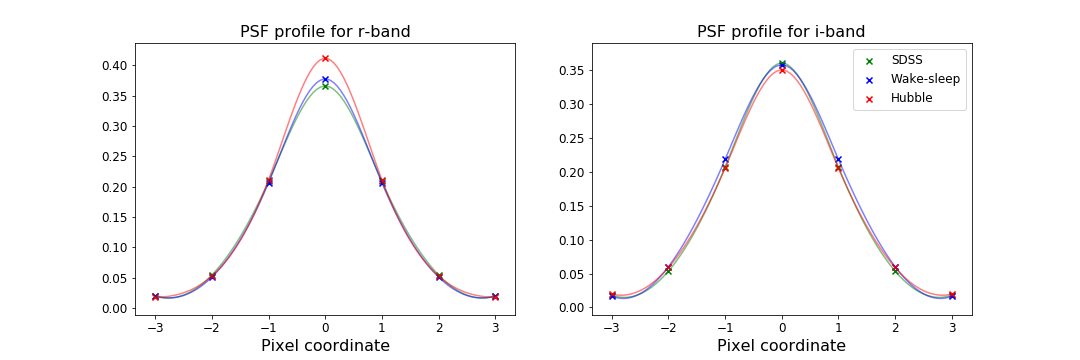
\includegraphics[width=0.99\textwidth]{figures/psf_profiles.png}
    \caption{Estimated versus true PSF profiles on M2. The Hubble PSF was
    obtained by optimizing the likelihood conditioned on locations and fluxes
    from the Hubble catalog. TODO: this image is not that informative, I think I'll remove this. }
    \label{fig:psf_profiles}
\end{figure}


% \multicolumn{1}{p{5cm}}{\raggedleft Neg. loglik \\ (with Hubble back.)}
% \caption{
% Chi-squared statistics for SDSS, wake-sleep, and Hubble estimated model parameters.
% The chi-squared statistic is defined as
% $\sum_{bij}\frac{([\text{obs.image}]_{bij} - [\text{recon.image}]_{bij})^2}{[\text{recon.image}]_{bij}}$.
% In the middle column, ``model parameters" refer to both background and PSF.
% In the right column, we fix the background to the Hubble estimate, and examine
% chi-squared statistics as the PSF varies.}

